% !TeX spellcheck = en_US
% !TEX root = ../thesis-example.tex
%
\section{Virtual Z Sorting}

We have now a properly keyed video feed and synchronous motion between a VR 
actor and the 3D environment. To increase the immersion of that composition the 
next important step is to sort the scene on a tri-graph of planes with a fore- 
and background - in between are frames from the motion video feed.

\begin{figure}[h]
	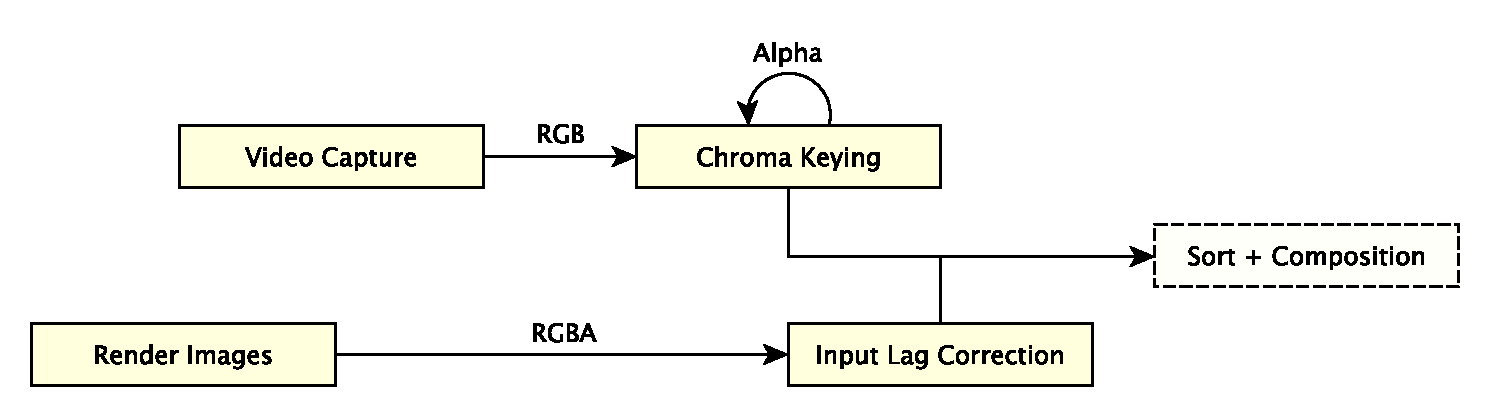
\includegraphics[width=\textwidth]{gfx/pipeline/4_5_composition.pdf}
	\caption{Current steps taken through the graphics pipeline}
	\label{fig:steps:composition}
\end{figure}

There are multiple ways to achieve proper segmentation and composition of all 
three layers, depending on the rendering method. Deferred shading allows for 
better lightning simulation in-engine but changes alpha- and depth maps of a 
rendered scenery - this yields incorrect layer blending and results into an 
incorrectly displayed image. This software takes account for this and lets 
visual artists decide between two render modes:

\begin{my_list}
	\item Replace Masking: A front plane is displayed, after it follows a 
	chroma-keyed video and then the background. This is the most accurate image 
	generation, if the front image is generated correctly and not modified by 
	post effects.
	\item Alpha Masking: A front alpha mask of the geometry is being generated, 
	then the actor is mixed with a full render image of the scenery's
	background. The resulting image has inconsistencies with alpha-blending but 
	this method works with all rendering setups.
\end{my_list}

\begin{figure}[htb]
	\includegraphics[width=\textwidth]{gfx/tri-graph.png}
	\caption{A sketch of the video composition with three layers of projection}
	\label{fig:zsort:sketch}
\end{figure}

The decision is between accuracy and presentation. Many post processing effects 
or deferred shading paths are unable --- or simply do not respect --- the 
alpha matte, which is usually no issue, since these steps are taken after 
rendering is complete, thus causing no unwanted side-effects in regular 
rendering pipelines. Other post effects need certain projection requirements 
and / or get discarded through culling, like in Figure 
\ref{fig:zsort:comparison}d where the volumetric lightning is culled out of the 
virtual projection and therefore gets completely ignored by the attached 
compute shader, resulting in a black, unlit front geometry because the light 
source is outside of the virtual cameras frustum.

\begin{figure}[htbp]
	\caption{A comparison of different composition methods in engine}
	\label{fig:zsort:comparison}
	\centering
	\begin{subfigure}[t]{.45\textwidth}
		\centering
		\includegraphics[width=\textwidth]{gfx/composition/Composition-Chroma-Result.png}
		\caption{The chroma keying result}
	\end{subfigure}
	\begin{subfigure}[t]{.45\textwidth}
		\centering
		\includegraphics[width=\textwidth]{gfx/composition/Composition-Full-Render.png}
		\caption{The full length rendering}
	\end{subfigure}
	\begin{subfigure}[t]{.45\textwidth}
		\centering
		\includegraphics[width=\textwidth]{gfx/composition/Composition-Perfect-Realigned.png}
		\caption{The proposed composition, simulated, with an arbitrary depth 
			of the video feed}
	\end{subfigure}
	\begin{subfigure}[t]{.45\textwidth}
		\centering
		\includegraphics[width=\textwidth]{gfx/composition/Composition-Front.png}
		\caption{The virtual projection of the front camera - volumetric 
			lightning does not work due to the short projection length}
		\end{subfigure}
	\begin{subfigure}[t]{.45\textwidth}
		\centering
		\includegraphics[width=\textwidth]{gfx/composition/Composition-Front-Replace_orso.png}
		\caption{A composition by rendering a front, followed by the video and 
		then the background}
	\end{subfigure}
	\begin{subfigure}[t]{.45\textwidth}
		\centering
		\includegraphics[width=\textwidth]{gfx/composition/Composition-Front-Mask.png}
		\caption{A composition with the front geometry as mask, and then a 
		mixing of the video and a full length render}
	\end{subfigure}
\end{figure}

Mixing these three layers is similarly effortless, using the previously 
established matting equation \eqref{eq:chroma:assumption:alpha:weak} and 
\eqref{eq:chroma:assumption:alpha:cont}. Assuming an ARGB front render image 
$C_F$, a RGB video feed  $C_V$ and the RGB background $C_B$, 
we can mix all three layers:

Replace Masking:

\eq{eq:zsort:replmask:1}{
	\alpha_{C_T} = \alpha_{C_V} * (1 - \alpha_{C_F})
}


\eq{eq:zsort:replmask:2}{
	I_{x, y} = (1 - \alpha_{C_T}) * C_{F_{x, y}} + \alpha_{C_T} * V_{x, y}
}

\eq{eq:zsort:replmask:3}{
	\alpha_{C_S} = \alpha_{C_B} * (1 - \alpha_{I_{x, y}})
}


\eq{eq:zsort:replmask:4}{
	J_{x, y} = (1 - \alpha_{C_S}) * I(x, y) + \alpha_{C_S} * C_{B_{x, y}}
}

Alpha Masking is very similar by transferring the alpha mask on the webcam 
footage after chroma-keying it. It is masking the video further, after the 
video matte is pulled already:

\eq{eq:zsort:alphamask:1}{
	\alpha_{V_T} = 
	\begin{cases}
		1 - \alpha_{C_F}  & \quad \text{if } \alpha_{C_V} > 0 \\
		\alpha_{C_V}      & \quad \text{otherwise}
	\end{cases}	
}

\eq{eq:zsort:alphamask:2}{
	\alpha_{C_T} =  \alpha_{C_B} * (1 - \alpha_{C_{V_T}})
}

\eq{eq:zsort:alphamask:3}{
	I_{x, y} = (1 - \alpha_{C_T}) * C_{V_{x, y}} + \alpha_{C_T} * C_{B_{x, y}}
}

We have a well-mixed image composition where the actor is placed in between 
two projection planes and thus can have an interactive fore- and background. 
The initial assumption is that the actor's depth is flattened to a plane, based 
on the distance between a real-world camera and the Vive Head Mounted Display.